Reduzieren Sie das folgende Problem auf das Halteproblem.

\begin{quote}
Gegeben ist eine Turing-Maschine $M$ und ein Wort $w$ auf dem Band.
Entscheide, ob die Turing-Maschine während ihrer Laufzeit den 
Bereich des Bandes verlässt, der $|w|$ Zeichen vor dem ersten
Zeichen von $w$ beginnt und $|w|$ Zeichen nach dem letzten Zeichen
von $w$ endet.
\end{quote}

\begin{center}
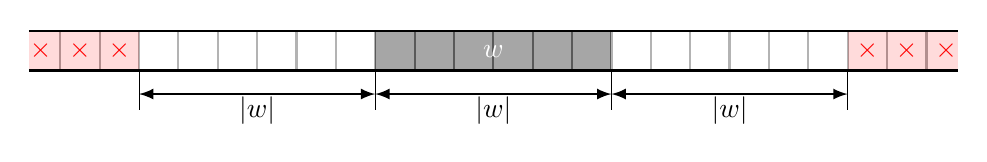
\begin{tikzpicture}[>=latex,thick]
\foreach \x in {0,0.5,...,11}{
	\draw (\x,0) -- (\x,0.5);
}
\foreach \x in {1,4,7,10}{
	\draw[line width=0.2pt] (\x,-0.5) -- (\x,0);
}
\draw[<->] (1,-0.3) -- (4,-0.3);
\draw[<->] (4,-0.3) -- (7,-0.3);
\draw[<->] (7,-0.3) -- (10,-0.3);
\node at (2.5,-0.2) [below] {$|w|$};
\node at (5.5,-0.2) [below] {$|w|$};
\node at (8.5,-0.2) [below] {$|w|$};
\begin{scope}
\clip (-0.4,0) rectangle (11.4,0.5);
\fill[color=red!20,opacity=0.7] (-0.4,0) rectangle (1,0.5);
\fill[color=white,opacity=0.7] (1,0) rectangle (4,0.5);
\fill[color=gray,opacity=0.7] (4,0) rectangle (7,0.5);
\fill[color=white,opacity=0.7] (7,0) rectangle (10,0.5);
\fill[color=red!20,opacity=0.7] (10,0) rectangle (11.4,0.5);
\foreach \x in {0.75,0.25,-0.25,10.25,10.75,11.25}{
	\node[color=red] at (\x,0.25) {$\times$};
}
\end{scope}
\node[color=white] at (5.5,0.25) {$w\mathstrut$};
\draw (-0.4,0) -- (11.4,0);
\draw (-0.4,0.5) -- (11.4,0.5);
\end{tikzpicture}
\end{center}


\begin{loesung}
Man könnte dem Bandalphabet ein neues Zeichen $\color{red}\times$
hinzufügen und es in die erste Zelle ausserhalb des zulässigen 
Bereiches schreiben.
Der Zustandsmaschine der Turing-Maschine fügen wir in jedem Zustand
einen Übergang nach $q_{\text{reject}}$ hinzu, wenn das aktuell Zeichen
ein ${\color{red}\times}$ ist.
Alle anderen Übergänge in Akzeptierzustände werden ersetzt durch einen
Übergang in eine Endlosschleife.
Damit wird aus der Turing-Maschine $M$ eine, die genau dann anhält,
wenn sie den erlaubten Bereich verlässt.

Etwas ähnliches kann man mit einem Debugger erreichen.
Man lädt das Programm in den Debugger und legt fest, dass
der Debugger anhalten soll, wenn es ausserhalb des erlaubten Bereiches
zugreiffen will.
Die Kombination Debugger mit geladenem Programm ist dann ein neues
Programm, welches anhält, wenn das ursprüngliche Programm den zulässigen
Bereich verlässt.

Real existierende Betriebssysteme lösen dieses Problem natürlich in 
Hardware.
Die Memory-Management-Unit des Prozessors detektiert, wenn ein
Speicherzugriff ausserhalb des allozierten oder erlaubten Bereiches ist 
und erzeugt einen Trap, der das Betriebssystem in die Lage versetzt,
das Problem zu behandeln.
\end{loesung}
